% !TEX root = ../thesis.tex
\chapter{Methodology}
\label{sec:methodology}
This chapter will outline the complete pipeline of our methodology.
It describes the process of data gathering and preprocessing,
with a focus on handling bias causing attributes.
The chapter then explains how the initial ML model is trained,
followed by the application of knowledge distillation to create an interpretable
representation of the model, which can then be modified to address unwanted biases.
The methodology further includes how the predictions of the modified representation
can be used to finetune the original model in order to improve fairness, while maintaining accuracy.

\section{Data Gathering}
Public real life event logs
containing sensitive attributes are hard to come by.
Additionally, in order to properly highlight the full capacity of our method,
we require the data to have sensitive attributes
that cause both positive and negative bias respectively.
Although \cite{simulated_logs} recently published simulated event logs,
seeking to address the scarcity of fairness-aware datasets in PBPM,
those event logs didn't show the structure we were looking for in this thesis.
Therefore, we will create the necessary data ourselves,
either by simulating a process or by enriching a real life event log with sensitive attributes.

\subsection{Event Log Simulation}
Our simulated event logs are generated by following rule-based transitions within a constructed process model.
Each case starts at an initial activity and progresses through sequential transitions to the next activity,
following the predefined sequence flow until reaching the end.
When reaching a gateway, the transition probabilities are determined by the values of the case attributes.
These values are being generated randomly for each process instance.
Additionally, for each transition, there is a $1\%$ chance that the process will deviate to a randomly selected activity,
even if there is no connecting sequence flow to that activity
This introduces variability and some realism into the simulation by occasionally branching out from the standard sequence of activities.
The timestamps in the simulated data do not convey meaningful information.
Instead, the time intervals between activities are randomly assigned between one and ten minutes.

An example of a simple process model, describing the treatment of patients in a hospital, is shown in Figure \ref{fig:showcase}.
This model consists of only four activities and uses \textit{gender} as its only case attribute.
The attribute \textit{gender} can take one of two values, \textit{male} or \textit{female}, each with an equal probability of 50\%.
In this example, \textit{gender} determines the probabilities at the gateway following the activity \textit{register patient}.
For \textit{male} patients, the probability of transitioning to \textit{regular treatment} is 70\%,
while the probability of transitioning to \textit{expert treatment} is 30\%.
Conversely, for \textit{female} patients, the probability of transitioning to \textit{regular treatment} is 30\%,
and the probability of transitioning to \textit{expert treatment} is 70\%.

\begin{figure}[h!]
    \centering
    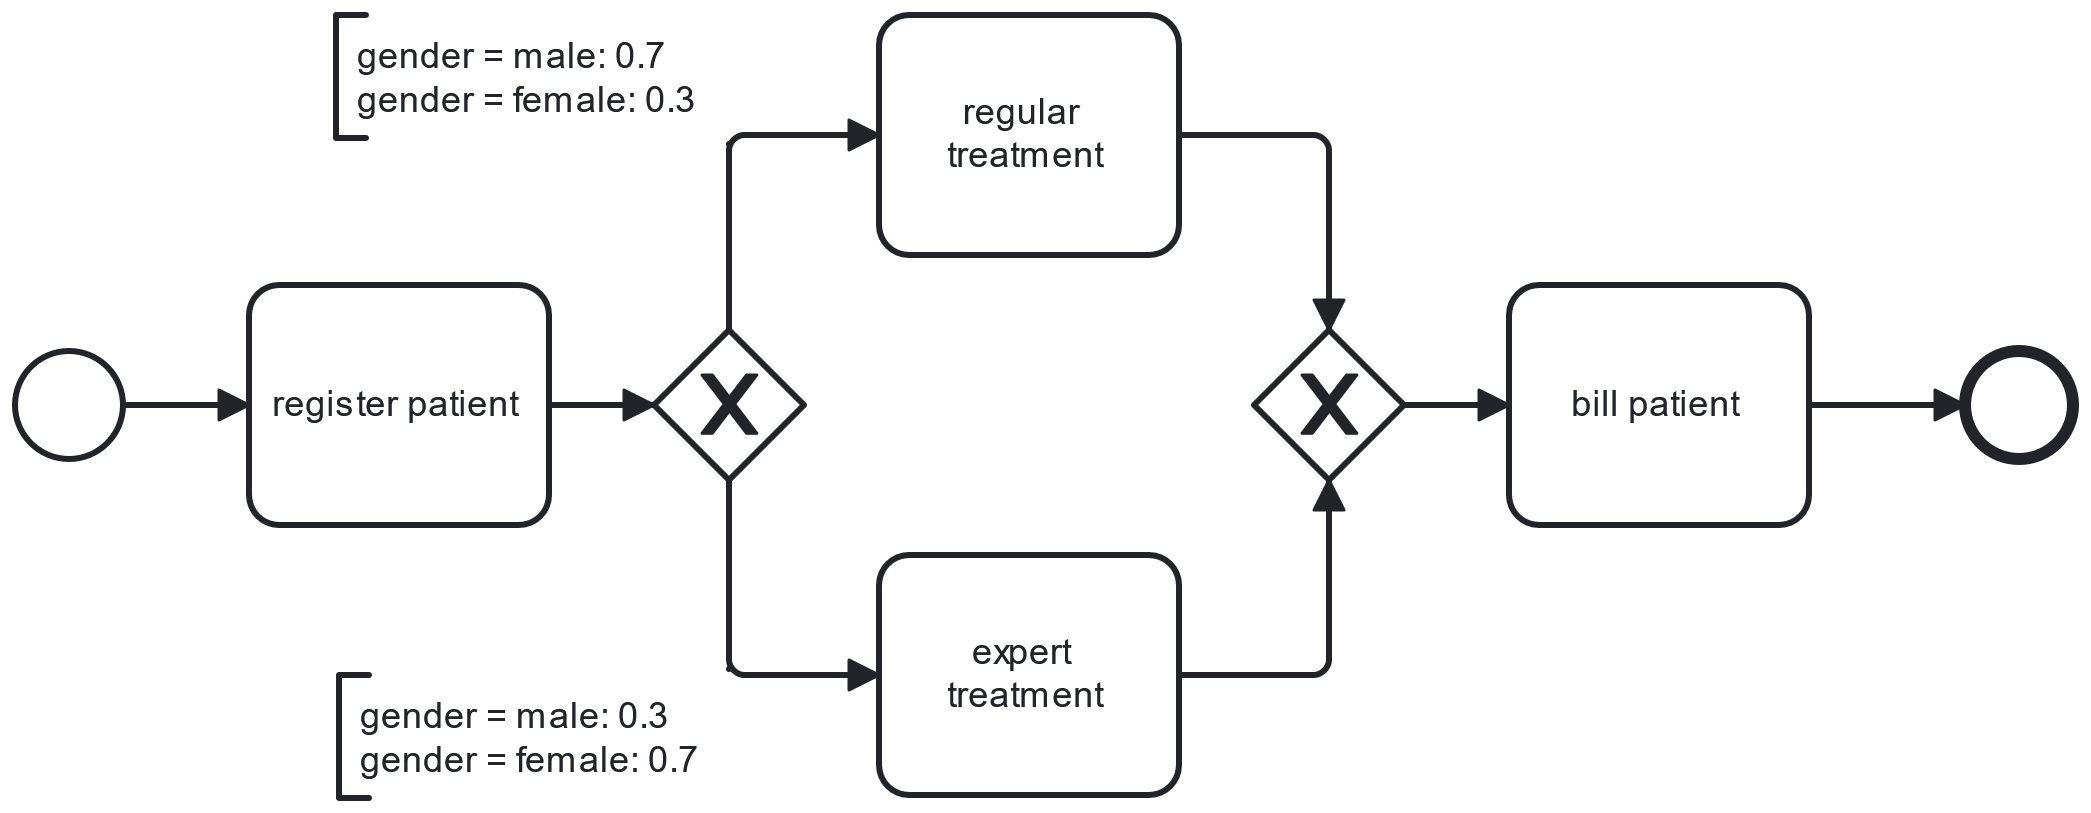
\includegraphics[width=\textwidth]{gfx/showcase.png}
    \caption{A simplified process model in BPMN describing the treatment of patients in a hospital, as portrayed before in Figure \ref{fig:bpmn_example}.
    The branches of the gateway are annotated with transition probabilities based on the case attribute \textit{gender}.
    We will use it as an example again in this chapter.}
    \label{fig:showcase}
\end{figure}


\subsection{Event Log Enrichment}
A common critique of using simulated event logs
is that their complexity may not fully reflect that of event logs derived from real-life processes.
To address this, we also augment publicly available event logs, which lack sensitive attributes,
by adding these attributes ourselves.
This enrichment process follows a set of predefined probabilistic rules,
that depend on the sequence of events observed in a case.
The case attributes are then assigned according to the distributions that aligns with the first matching rule.
Detailed examples of these enrichment rules
and their corresponding attribute distributions are provided in chapter \ref{sec:evaluation}.

\section{Preprocessing}
\label{sec:preprocessing}
Since NNs cannot learn from the event log format directly,
we preprocess the data to generate samples in the form of $(x,y)$,
where $x = (x_1, ..., x_n)$ represents the $n$ input features and $y = (y_1, ..., y_k)$ represents the target outcome
out of $k$ activities, as described in section \ref{sec:backpropagation}. 
In order to do this, we extract all possible prefix-outcome pairs from each case in the event log.
The prefix consists of the sequence of events up to a certain point in the case,
while the outcome corresponds to the next activity after the prefix.
Our target $y$ can be directly derived from the next activities by one-hot encoding.

The input $x$ should contain information about both the prefix and the corresponding case attributes.
Since neural networks require inputs of a fixed size,
we handle the varying lengths of prefixes by applying a sliding window of a static size $w$.
If a prefix is shorter than the window size,
we pad the sequence with a special \textit{<PAD>} activity to fill the remaining positions.
Conversely, if a prefix is longer than $w$, we truncate it to include only the most recent $w$ events. 

Case attributes are encoded based on their type.
Categorical attributes are one-hot encoded in the same way as activities,
ensuring that each category is represented as a unique vector.
For consistency purposes, we will also one-hot encode categorical attributes that have only two possible values,
even though a single bit would suffice for 
Numerical attributes are normalized using \textbf{min-max scaling},
which rescales their values to fall within the range of 0 to 1,
ensuring that all attributes contribute equally to the model's training process,
preventing numerical attributes with larger magnitudes from dominating those with smaller ones,
as well as categorical attributes.
Given a numerical value $z$, the scaled value $z'$ is calculated as 
\begin{align}
    z' = \frac{z - \textit{min}}{\textit{max} - \textit{min}}
\end{align}
where \textit{min} and \textit{max} refer to the minimum and maximum observed values of the attribute in the dataset.
Finally, we concatenate the sequence of one-hot encoded activities
and the encoded case attributes into the input vector $x$.

\begin{table}[h!]
    \centering
    \scriptsize
    \renewcommand{\arraystretch}{1.2}
    \setlength{\tabcolsep}{6pt}

    \begin{minipage}{0.55\textwidth}
        \centering
        \begin{tabular}{c | c}
            \toprule
            \textbf{Previous Activity} & \textbf{Encoding} \\
            \midrule
            <PAD> & [\textcolor{blue}{1}, \textcolor{blue}{0}, \textcolor{blue}{0}, \textcolor{blue}{0}, \textcolor{blue}{0}] \\
            register patient & [\textcolor{blue}{0}, \textcolor{blue}{1}, \textcolor{blue}{0}, \textcolor{blue}{0}, \textcolor{blue}{0}] \\
            regular treatment & [\textcolor{blue}{0}, \textcolor{blue}{0}, \textcolor{blue}{1}, \textcolor{blue}{0}, \textcolor{blue}{0}] \\
            expert treatment & [\textcolor{blue}{0}, \textcolor{blue}{0}, \textcolor{blue}{0}, \textcolor{blue}{1}, \textcolor{blue}{0}] \\
            bill patient & [\textcolor{blue}{0}, \textcolor{blue}{0}, \textcolor{blue}{0}, \textcolor{blue}{0}, \textcolor{blue}{1}] \\
            \bottomrule
        \end{tabular}
    \end{minipage}
    %\hspace{0.5cm}
    \begin{minipage}{0.3\textwidth}
        \centering
        \vspace{0.2cm}
        \begin{tabular}{c | c}
            \toprule
            \textbf{Gender} & \textbf{Encoding} \\
            \midrule
            male & [\textcolor{red}{1}, \textcolor{red}{0}] \\
            female & [\textcolor{red}{0}, \textcolor{red}{1}] \\
            \bottomrule
        \end{tabular}
    \end{minipage}

    \vspace{0.3cm}

    \begin{minipage}{0.7\textwidth}
        \centering
        \begin{tabular}{c | c | c | c | c}
            \toprule
            \textbf{Previous Activity} & \textbf{Gender} & \textbf{Next Activity} & \textbf{x Encoding} & \textbf{y Encoding} \\
            \midrule
            register patient & male & expert treatment & 
            [\textcolor{blue}{0}, \textcolor{blue}{1}, \textcolor{blue}{0}, \textcolor{blue}{0}, \textcolor{blue}{0}, \textcolor{red}{1}, \textcolor{red}{0}] & 
            [\textcolor{blue}{0}, \textcolor{blue}{0}, \textcolor{blue}{0}, \textcolor{blue}{1}, \textcolor{blue}{0}] \\
            
            expert treatment & male & bill patient & 
            [\textcolor{blue}{0}, \textcolor{blue}{0}, \textcolor{blue}{0}, \textcolor{blue}{1}, \textcolor{blue}{0}, \textcolor{red}{1}, \textcolor{red}{0}] & 
            [\textcolor{blue}{0}, \textcolor{blue}{0}, \textcolor{blue}{0}, \textcolor{blue}{0}, \textcolor{blue}{1}] \\
            
            register patient & female & regular treatment & 
            [\textcolor{blue}{0}, \textcolor{blue}{1}, \textcolor{blue}{0}, \textcolor{blue}{0}, \textcolor{blue}{0}, \textcolor{red}{0}, \textcolor{red}{1}] & 
            [\textcolor{blue}{0}, \textcolor{blue}{0}, \textcolor{blue}{1}, \textcolor{blue}{0}, \textcolor{blue}{0}] \\
            \bottomrule
        \end{tabular}
    \end{minipage}

    \vspace{0.2cm}

    \caption{Tables portraying the one-hot encoding of the previous activities (top left) and genders (top right),
    as well as the input-output mappings for some samples from the model presented in Figure \ref{fig:showcase} (bottom).
    }
    \label{tab:preprocessing}
\end{table}


After processing all samples, we have to consider how to split the samples into a \textbf{training set} and a \textbf{test set}.
The training set is used to improve the NN's accuracy,
while the test set is reserved for the final evaluation of the model's performance after training is complete.
It is crucial to keep these sets strictly separated to prevent any information
from the test set leaking into the training set.
Therefore, special care must be taken during the splitting process: \cite{data_split}

\begin{itemize}
\item \textbf{Min-Max Scaling:}  
When performing min-max scaling,
the scaling parameters min and max are derived from just the training set.
This simulates a real-world scenario in which only the values of old training data is known to us,
which ensures that the test set remains independent.
\item \textbf{Instance-Level Leakage:}  
We ensure that all events of a single case are contained either in the training set or the test set, but not both.
Splitting process instances across sets might lead to information leakage,
allowing the model to gain knowledge about test data it would not have access to in a real-world scenario.
\item \textbf{Temporal Leakage:}  
When utilizing timestamp date, one could consider using a chronological split to train on earlier cases and test on later ones.
This setup mimics real-world predictive scenarios where historical data is used to predict outcomes for future events.
In our case, we mostly use simulated event logs, in which there is no chronological difference,
or public event logs, in which the timestamps have been anonymized,
maintaining only the time difference between events. \cite{hospital_billing}
Therefore, a random split can be used instead.
\item \textbf{Cluster Leakage:}  
If the dataset contains groups of highly similar cases, e.g., cases grouped by customer, department, or product line,
assigning entire clusters to either the training or test set prevents correlated information from leaking between the splits.
The datasets we use however are either simulated or anonymized to protect personal information \cite{hospital_billing}.
As a result, no distinct clusters are evident, making a random split both appropriate and sufficient.
\item \textbf{Representative Datasets:}  
Lastly, it's important to ensure that the test set is representative of the dataset's overall diversity.
Specifically, one should avoid creating splits where rare or common cases are disproportionately represented in one set,
as this could skew model evaluation and lead to biased results.
Since we are working with rather large datasets, any bias introduced by random splitting is likely to be minimal.
Moreover, our primary objective is not to achieve maximum accuracy but to enable a fair and consistent comparison between models,
making randomly splitting acceptable for this task.
\end{itemize}

\section{Training the Neural Network}
\label{sec:training}
After processing the event log into a dataset suitable for machine learning,
we proceed to train a feedforward neural network (NN) using the prepared samples.
The model is implemented using the the Keras \cite{keras} library,
which allows for a straightforward layer-by-layer construction of the network.
As mentioned earlier, our primary focus is not on fully optimizing accuracy,
so we did not invest extensive time or effort into selecting and fine-tuning the model's hyperparameters.
The following architecture and hyperparameters were chosen, because they delivered consistently good results in practice:

The NN incorporates four hidden layers with 512, 256, 128, and 64 neurons
The choice of progressively smaller layer sizes allows the network to gradually distill
the input features into more abstract representations, facilitating the learning of hierarchical patterns. 
The amount of perceptrons in the input and output layer is dependent on the task at hand,
determined by the dimensions of the processed input and output samples respectively.
The hidden layer uses the ReLU activation function,
while the ouput layer uses softmax activation, as described in section \ref{sec:feedforward}.

For the training process, we used categorical cross-entropy loss in conjunction with the Adam optimizer,
utilizing its default parameters as provided by Keras, with a learning rate of $\alpha = 0.001$.
The model is trained for a total of 10 epochs, with a batch size of 32.
In our experiments, 10 epochs were sufficient for the model to converge without overfitting.
The batch size of 32 was chosen because it offers a practical compromise
between computational efficiency and stable gradient updates.
This configuration enabled the model to learn effectively
and produce satisfactory results within a reasonable training time.

\section{Knowledge Distillation}
After training, the NN is expected to achieve high accuracy but may produce biased predictions,
hidden by its black-box nature.
To uncover these biases and better understand the NN's inner workings,
we train a transparent model that mimics the NN's behavior.

This approach leverages \textbf{knowledge distillation},
a technique originally developed to transfer knowledge from a large,
complex model \textbf{(teacher)} to a smaller,
more efficient model \textbf{(student)} \cite{knowledge_distillation}.
By training the student to replicate the teacher's outputs instead of the original training targets,
knowledge distillation enables faster inference and reduced computational demands,
while preserving predictive performance.
In addition to efficiency, knowledge distillation has been adapted for interpretability
by training a white-box student model to approximate the teacher model's predictions. \cite{knowledge_distillation_trees}
This allows the decision-making process of the opaque NN
to be examined through the interpretable structure of the student,
providing insights into its behavior while retaining much of its predictive accuracy.

We opted to use regular decision trees (DTs) as defined in section \ref{sec:dt},
since they are both easy to implement and can be interpreted well
even by domain experts not too familiar in the field of machine learning.
However, DTs cannot directly utilize the softened output $\hat{y}$ produced by the softmax activation
in the output layer of the neural network,
as they require discrete class labels rather than a probability distribution.
To address this, we apply the \textit{argmax} function to select the class index
with the highest probability from the distribution.
Formally, given a training sample $x$,
the distilled target labels $\bar{y}$ are derived from the NN's output as follows:
\begin{align}
    \bar{y} = \textit{argmax}(\textit{NN}(x))
\end{align}


\section{Training the Decision Tree}
Using the input samples $x$ from the training dataset
and their corresponding distilled target samples $\bar{y}$ from the NN, we proceed to train our DT.
For this, we employ the \textbf{DecisionTreeClassifier} class from the Sklearn library \cite{sklearn},
utilzing its default parameters for training.
As outlined in section \ref{sec:dt_training},
the DT is constructed by recursively partitioning the training dataset at each node to minimize Gini impurity,
until either all leaves contain pure target classes or until further splits no longer reduce impurity.

Additionally, minimal cost-complexity pruning is applied with $\alpha=0.001$,
eliminating splits that provide negligible reductions in impurity.
Selecting an appropriate $\alpha$ is important, as excessivly larger values may remove important nodes that rely on sensitive attributes, making it impossible to modify the tree structure as intended.
A more robust approach would involve computing the cost-complexity pruning path by iteratively increasing $\alpha$ and recording the sequence of pruned subtrees.
This process generates a series of increasingly simplified trees, each corresponding to a different value of $\alpha$.
The optimal subtree is then selected based on a validation criterion, such as minimizing prediction error.
However, due to computational constraints and the fact that the results were satisfactory without fine-tuning $\alpha$, we opted for a fixed value instead.


\section{Modification of the Decision Tree}
\label{sec:modification}
Now that the inner workings of the NN have been represented as a decision tree,
we can examine its structure for potential biases.
Specifically, we look for inner nodes that use sensitive attributes as the basis for their splits
and assess whether such usage is justified in the context of the node.
If we determine that one or more nodes unfairly rely on sensitive attributes,
we can modify the decision tree structure by deleting those biased nodes,
thereby removing their influence.
To remove a biased node $v$ while maintaining the defined structure of a binary DT,
we have several possible options:

\begin{itemize}
    \item \textbf{Cutting Branches:} 
    Let $u_1, u_2$ be the children of $v$ and $|S_{u_1}|, |S_{u_2}|$
    the number of training samples associated with each child respectively.
    When removing the node $v$ from the tree,
    the simplest approach would be to replace $v$ with the child node $u_i$
    that has more associated training sampels $|S_{u_i}|$, with $i \in \{1,2\}$.
    Basically, we would eliminate the subtree rooted at the child with less samples.
    This method ensures that the majority of samples are still handled similarly,
    while removing the biased split from the DT.
    However, the subtree and its splits may lose their coherence without the biased split,
    potentially leading to a significant drop in predictive performance after the modification.

    \item \textbf{Retraining Subtrees:}
    An alternative approach when removing $v$ is to delete the entire subtree rooted at $v$
    and retrain it using the samples associated with $v$.  
    The retraining process follows the procedure outlined in section \ref{sec:dt_training},
    stopping when the dataset becomes fully pure or when the retrained subtree reaches a greater depth than the
    subtree rooted at $v$ had before.  
    To prevent the retrained subtree from making the same biased split however,
    any features related to the sensitive attributes used by $v$ must be excluded from the entire subtree.  
    Although this results in more coherent splits,
    there is a possibility that the sensitive attribute could have been used by a descendant of $v$ in a beneficial way,
    which we might not want to eliminate.
    Additionally, the retraining process could introduce new biases related to other sensitive attributes that were not previously present.  
    This means the retraining may need to be repeated multiple times until all unwanted bias is removed.  

    \item \textbf{Manual Modification:}  
    Finally, a domain expert could manually modify the decision tree, its node structure,
    and the associated features and thresholds based on their understanding of how the splits should be structured.
    However, even with domain knowledge,
    manually adjusting the decision tree requires significant effort
    and is challenging to do without substantially compromising prediction accuracy.
\end{itemize}

\begin{figure}[h!]
    \centering
    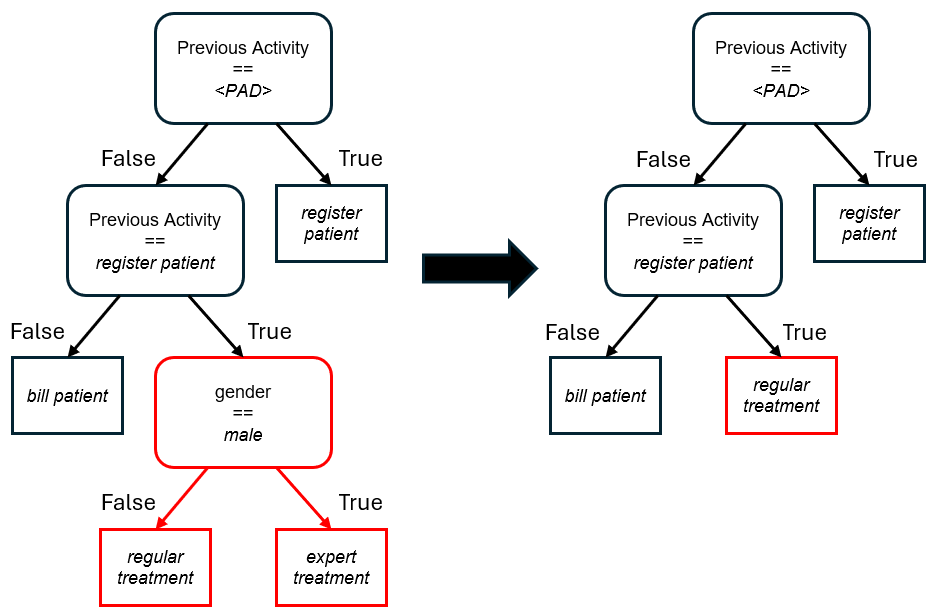
\includegraphics[width=\textwidth]{gfx/modification.png}
    \caption{Two DTs suitable for next activity prediction in the process model shown in Figure \ref{fig:showcase}.
    The DT on the left represents the original model, which uses gender discriminatingly in the subtree highlighted in red.
    Since no alternative attribute is available for making this decision,
    one possible modification to improve fairness would be to remove the branch leading to \textit{expert treatment},
    resulting in the modified DT on the right.
    }
    \label{fig:modification}
\end{figure}

\section{Finetuning of the Model}
By modifying the DT, our goal was to obtain a predictor that 
makes fairer decisions, while maintaining most of the NN's predictive power.
While we could just use the DT directly for the task of next activity prediction,
deep learning methods generally outperform traditional machine learning approaches,
when it comes to solving complex tasks \cite{ml_comparison}.
In order to combine the more precise predictions of the NN with the fairer decisions of the DT,
we attempt to fine-tune our NN in accordance to the predictions of the modified DT.

Generally speaking, \textbf{fine-tuning} \cite{fine_tuning} is a transfer learning technique
that involves adapting a pre-trained model to a new task or dataset.
Rather than training a neural network from scratch,
fine-tuning starts with a model that has already been trained on a related task,
leveraging its pre-learned features.
This reduces training time, requires fewer data, and often improves performance
by building on the general representations learned during pre-training.

In our case, we fine-tune the pre-trained NN from the previous section \ref{sec:training},
using a training set that was modified to increase group fairness.
This fine-tuning dataset retains the same input samples $x$ from the original training set,
but leverages the outputs from the modified DT to replace the original targets $y$.
However, we cannot utilize the immediate output of the modified DT directly, since NNs require distributions as their targets,
instead of the discrete labels provided by the DT.
To address this, we apply one-hot encoding to the output of the modified DT,
receiving a vector $\tilde{y}$ for a training sample $x$ as follows:
\begin{align}
    \tilde{y} = \textit{one-hot}(\textit{DT}_{mod}(x))
\end{align}

When selecting appropriate targets for the training set during fine-tuning,
we explored several strategies.
The following two approaches yielded the best results in our experiments:

\begin{itemize}  
    \item \textbf{Full Correction}:  
    In the first approach, the NN is trained to directly mimic the modified DT by using $\tilde{y}$ as the new training target for all samples.
    This ensures that the NN fully inherits the fairness properties of the DT, but also means that any misclassifications made by the modified DT are learned as well,
    even if those are independent of the fairness concerns.
    As a result, the accuracy of the NN may decrease further than necessary. 

    \item \textbf{Selective Correction}:  
    An alternative approach selectively utilizes $\tilde{y}$ as targets only for samples where the modified DT's predictions differ from those of the original distilled DT.
    Otherwise, we retain the original NN's predictions as training targets, such that the learned parameters are being changed as little as possible.
    This method ensures that the NN specifically corrects unfair classifications that, thereby mitigating the risk of reduced accuracy caused by erroneous DT predictions.
\end{itemize}  

Although \textbf{selective correction} is usually the better choice, it doesn't perform better for all event logs we tested.
Therefore, when finetuning, we employ both described approaches and pick the one that yields the better accuracy results.
The training process during fine-tuning was similar to the initial training procedure
described in section \ref{sec:training}, with minor adjustments.
We did not conduct extensive tests regarding the fine-tuning hyperparameters,
since the ideal settings are heavily dependent on both the 
dataset and the architecture of the black-box predictor.
However, these selected hyperparameters yielded satisfactory results in our experiments:
We reduced the Adam optimizer's learning rate $\alpha$ from $0.001$
to $0.00001$ to balance fairness improvements with maintaining the pre-trained weights.
Additionally, the number of epochs was reduced from 10 to 5,
as the NN's accuracy converges quicker on the modified distilled targets.

%TODO: image: process - complete timeline?